\chapter{图的遍历}

本章讨论两种基本的图算法：
深度优先搜索和广度优先搜索。
这两种算法都从图中的一个起始节点出发，
访问所有可以从起始节点到达的节点。
它们之间的区别在于访问节点的顺序。

\section{深度优先搜索}

\index{深度优先搜索}

\key{深度优先搜索}（DFS）
是一种直观的图遍历技术。
该算法从一个起始节点出发，
沿着图的边前进，到达所有可以从
起始节点到达的其他节点。

深度优先搜索始终沿着图中的
一条路径不断前进，只要能找到
新的节点就继续下去。
之后，它返回之前的节点，
开始探索图的其他部分。
算法会记录已访问的节点，
因此每个节点只会被处理一次。

\subsubsection*{示例}

让我们来看看深度优先搜索如何处理
以下图：
\begin{center}
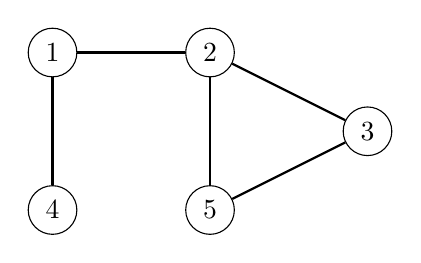
\begin{tikzpicture}
\node[draw, circle] (1) at (1,5) {$1$};
\node[draw, circle] (2) at (3,5) {$2$};
\node[draw, circle] (3) at (5,4) {$3$};
\node[draw, circle] (4) at (1,3) {$4$};
\node[draw, circle] (5) at (3,3) {$5$};

\path[draw,thick,-] (1) -- (2);
\path[draw,thick,-] (2) -- (3);
\path[draw,thick,-] (1) -- (4);
\path[draw,thick,-] (3) -- (5);
\path[draw,thick,-] (2) -- (5);
\end{tikzpicture}
\end{center}
我们可以从图中的任意节点开始搜索；
现在我们从节点 1 开始搜索。

搜索首先前进到节点 2：
\begin{center}
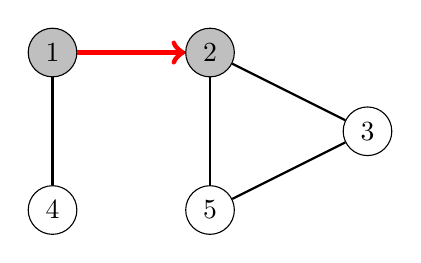
\begin{tikzpicture}
\node[draw, circle,fill=lightgray] (1) at (1,5) {$1$};
\node[draw, circle,fill=lightgray] (2) at (3,5) {$2$};
\node[draw, circle] (3) at (5,4) {$3$};
\node[draw, circle] (4) at (1,3) {$4$};
\node[draw, circle] (5) at (3,3) {$5$};

\path[draw,thick,-] (1) -- (2);
\path[draw,thick,-] (2) -- (3);
\path[draw,thick,-] (1) -- (4);
\path[draw,thick,-] (3) -- (5);
\path[draw,thick,-] (2) -- (5);

\path[draw=red,thick,->,line width=2pt] (1) -- (2);
\end{tikzpicture}
\end{center}
此后，节点 3 和 5 将被访问：
\begin{center}
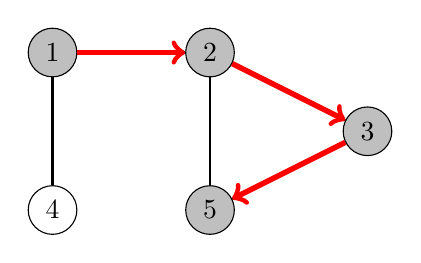
\begin{tikzpicture}
\node[draw, circle,fill=lightgray] (1) at (1,5) {$1$};
\node[draw, circle,fill=lightgray] (2) at (3,5) {$2$};
\node[draw, circle,fill=lightgray] (3) at (5,4) {$3$};
\node[draw, circle] (4) at (1,3) {$4$};
\node[draw, circle,fill=lightgray] (5) at (3,3) {$5$};

\path[draw,thick,-] (1) -- (2);
\path[draw,thick,-] (2) -- (3);
\path[draw,thick,-] (1) -- (4);
\path[draw,thick,-] (3) -- (5);
\path[draw,thick,-] (2) -- (5);

\path[draw=red,thick,->,line width=2pt] (1) -- (2);
\path[draw=red,thick,->,line width=2pt] (2) -- (3);
\path[draw=red,thick,->,line width=2pt] (3) -- (5);
\end{tikzpicture}
\end{center}
节点 5 的邻居是 2 和 3，
但搜索已经访问过这两个节点了，
所以是时候返回之前的节点了。
节点 3 和 2 的邻居也都已经被访问过了，
所以接下来我们从节点 1 移动到节点 4：
\begin{center}
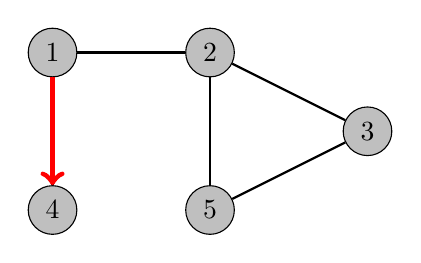
\begin{tikzpicture}
\node[draw, circle,fill=lightgray] (1) at (1,5) {$1$};
\node[draw, circle,fill=lightgray] (2) at (3,5) {$2$};
\node[draw, circle,fill=lightgray] (3) at (5,4) {$3$};
\node[draw, circle,fill=lightgray] (4) at (1,3) {$4$};
\node[draw, circle,fill=lightgray] (5) at (3,3) {$5$};

\path[draw,thick,-] (1) -- (2);
\path[draw,thick,-] (2) -- (3);
\path[draw,thick,-] (1) -- (4);
\path[draw,thick,-] (3) -- (5);
\path[draw,thick,-] (2) -- (5);

\path[draw=red,thick,->,line width=2pt] (1) -- (4);
\end{tikzpicture}
\end{center}
此后，搜索结束，因为所有节点
都已被访问。

深度优先搜索的时间复杂度为 $O(n+m)$，
其中 $n$ 是节点数，$m$ 是边数，
因为算法对每个节点和每条边都只处理一次。

\subsubsection*{实现}

深度优先搜索可以方便地
使用递归来实现。
以下函数 \texttt{dfs} 从给定节点
开始进行深度优先搜索。
该函数假设图以邻接表的形式
存储在一个数组中：
\begin{lstlisting}
vector<int> adj[N];
\end{lstlisting}
并且还维护一个数组
\begin{lstlisting}
bool visited[N];
\end{lstlisting}
用于记录已访问的节点。
初始时，每个数组值为 \texttt{false}，
当搜索到达节点 $s$ 时，
\texttt{visited}[$s$] 的值变为 \texttt{true}。
该函数可以实现如下：
\begin{lstlisting}
void dfs(int s) {
    if (visited[s]) return;
    visited[s] = true;
    // 处理节点 s
    for (auto u: adj[s]) {
        dfs(u);
    }
}
\end{lstlisting}

\section{广度优先搜索}

\index{广度优先搜索}

\key{广度优先搜索}（BFS）按照节点到
起始节点的距离递增的顺序访问节点。
因此，我们可以使用广度优先搜索
计算从起始节点到所有其他
节点的距离。
然而，广度优先搜索的实现
比深度优先搜索更复杂。

广度优先搜索逐层遍历节点。
首先搜索探索距离起始节点为 1 的节点，
然后是距离为 2 的节点，依此类推。
这个过程持续到所有节点
都被访问为止。

\subsubsection*{示例}

让我们来看看广度优先搜索如何处理
以下图：

\begin{center}
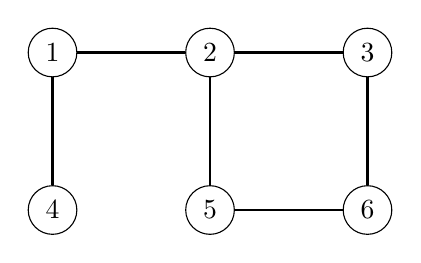
\begin{tikzpicture}
\node[draw, circle] (1) at (1,5) {$1$};
\node[draw, circle] (2) at (3,5) {$2$};
\node[draw, circle] (3) at (5,5) {$3$};
\node[draw, circle] (4) at (1,3) {$4$};
\node[draw, circle] (5) at (3,3) {$5$};
\node[draw, circle] (6) at (5,3) {$6$};

\path[draw,thick,-] (1) -- (2);
\path[draw,thick,-] (2) -- (3);
\path[draw,thick,-] (1) -- (4);
\path[draw,thick,-] (3) -- (6);
\path[draw,thick,-] (2) -- (5);
\path[draw,thick,-] (5) -- (6);
\end{tikzpicture}
\end{center}
假设搜索从节点 1 开始。
首先，我们处理所有可以从节点 1 
通过一条边到达的节点：
\begin{center}
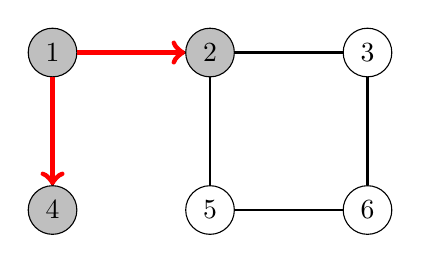
\begin{tikzpicture}
\node[draw, circle,fill=lightgray] (1) at (1,5) {$1$};
\node[draw, circle,fill=lightgray] (2) at (3,5) {$2$};
\node[draw, circle] (3) at (5,5) {$3$};
\node[draw, circle,fill=lightgray] (4) at (1,3) {$4$};
\node[draw, circle] (5) at (3,3) {$5$};
\node[draw, circle] (6) at (5,3) {$6$};

\path[draw,thick,-] (1) -- (2);
\path[draw,thick,-] (2) -- (3);
\path[draw,thick,-] (1) -- (4);
\path[draw,thick,-] (3) -- (6);
\path[draw,thick,-] (2) -- (5);
\path[draw,thick,-] (5) -- (6);

\path[draw,thick,-] (1) -- (2);
\path[draw,thick,-] (2) -- (3);
\path[draw,thick,-] (1) -- (4);
\path[draw,thick,-] (2) -- (5);

\path[draw=red,thick,->,line width=2pt] (1) -- (2);
\path[draw=red,thick,->,line width=2pt] (1) -- (4);
\end{tikzpicture}
\end{center}
此后，我们前进到节点 3 和 5：
\begin{center}
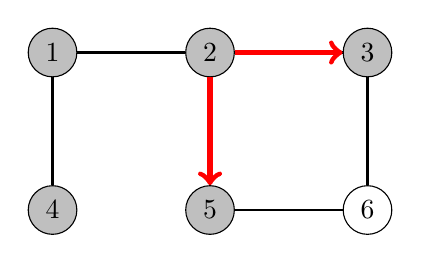
\begin{tikzpicture}
\node[draw, circle,fill=lightgray] (1) at (1,5) {$1$};
\node[draw, circle,fill=lightgray] (2) at (3,5) {$2$};
\node[draw, circle,fill=lightgray] (3) at (5,5) {$3$};
\node[draw, circle,fill=lightgray] (4) at (1,3) {$4$};
\node[draw, circle,fill=lightgray] (5) at (3,3) {$5$};
\node[draw, circle] (6) at (5,3) {$6$};

\path[draw,thick,-] (1) -- (2);
\path[draw,thick,-] (2) -- (3);
\path[draw,thick,-] (1) -- (4);
\path[draw,thick,-] (3) -- (6);
\path[draw,thick,-] (2) -- (5);
\path[draw,thick,-] (5) -- (6);

\path[draw,thick,-] (1) -- (2);
\path[draw,thick,-] (2) -- (3);
\path[draw,thick,-] (1) -- (4);
\path[draw,thick,-] (2) -- (5);

\path[draw=red,thick,->,line width=2pt] (2) -- (3);
\path[draw=red,thick,->,line width=2pt] (2) -- (5);
\end{tikzpicture}
\end{center}
最后，我们访问节点 6：
\begin{center}
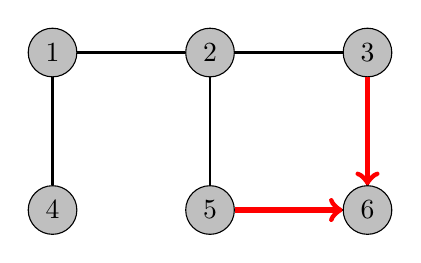
\begin{tikzpicture}
\node[draw, circle,fill=lightgray] (1) at (1,5) {$1$};
\node[draw, circle,fill=lightgray] (2) at (3,5) {$2$};
\node[draw, circle,fill=lightgray] (3) at (5,5) {$3$};
\node[draw, circle,fill=lightgray] (4) at (1,3) {$4$};
\node[draw, circle,fill=lightgray] (5) at (3,3) {$5$};
\node[draw, circle,fill=lightgray] (6) at (5,3) {$6$};

\path[draw,thick,-] (1) -- (2);
\path[draw,thick,-] (2) -- (3);
\path[draw,thick,-] (1) -- (4);
\path[draw,thick,-] (3) -- (6);
\path[draw,thick,-] (2) -- (5);
\path[draw,thick,-] (5) -- (6);

\path[draw,thick,-] (1) -- (2);
\path[draw,thick,-] (2) -- (3);
\path[draw,thick,-] (1) -- (4);
\path[draw,thick,-] (2) -- (5);

\path[draw=red,thick,->,line width=2pt] (3) -- (6);
\path[draw=red,thick,->,line width=2pt] (5) -- (6);
\end{tikzpicture}
\end{center}
现在我们已经计算出了
从起始节点到图中所有节点的距离。
距离如下：

\begin{tabular}{ll}
\\
节点 & 距离 \\
\hline
1 & 0 \\
2 & 1 \\
3 & 2 \\
4 & 1 \\
5 & 2 \\
6 & 3 \\
\\
\end{tabular}

与深度优先搜索一样，
广度优先搜索的时间复杂度
也是 $O(n+m)$，其中 $n$ 是节点数，
$m$ 是边数。

\subsubsection*{实现}

广度优先搜索比深度优先搜索更难实现，
因为算法会访问图中不同部分的节点。
一种典型的实现是基于一个包含节点的队列。
在每一步中，队列中的下一个节点
将被处理。

以下代码假设图以邻接表的形式存储，
并维护以下数据结构：
\begin{lstlisting}
queue<int> q;
bool visited[N];
int distance[N];
\end{lstlisting}

队列 \texttt{q}
包含待处理的节点，
按其距离递增的顺序排列。
新节点总是被添加到队列的末尾，
而队列开头的节点是下一个要处理的节点。
数组 \texttt{visited} 表示
搜索已经访问过哪些节点，
数组 \texttt{distance} 将包含
从起始节点到图中所有节点的距离。

搜索可以实现如下，
从节点 $x$ 开始：
\begin{lstlisting}
visited[x] = true;
distance[x] = 0;
q.push(x);
while (!q.empty()) {
    int s = q.front(); q.pop();
    // 处理节点 s
    for (auto u : adj[s]) {
        if (visited[u]) continue;
        visited[u] = true;
        distance[u] = distance[s]+1;
        q.push(u);
    }
}
\end{lstlisting}

\section{应用}

利用图的遍历算法，
我们可以检查图的许多性质。
通常，深度优先搜索和广度优先搜索都可以使用，
但在实践中，深度优先搜索
是更好的选择，因为它更容易实现。
在以下应用中，我们假设图是无向图。

\subsubsection{连通性检查}

\index{连通图}

如果一个图中任意两个节点之间都存在路径，
则该图是连通的。
因此，我们可以通过从任意节点出发，
检查是否能到达所有其他节点，
来判断一个图是否是连通的。

例如，在图
\begin{center}
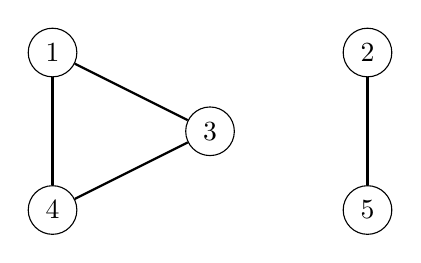
\begin{tikzpicture}
\node[draw, circle] (2) at (7,5) {$2$};
\node[draw, circle] (1) at (3,5) {$1$};
\node[draw, circle] (3) at (5,4) {$3$};
\node[draw, circle] (5) at (7,3) {$5$};
\node[draw, circle] (4) at (3,3) {$4$};

\path[draw,thick,-] (1) -- (3);
\path[draw,thick,-] (1) -- (4);
\path[draw,thick,-] (3) -- (4);
\path[draw,thick,-] (2) -- (5);
\end{tikzpicture}
\end{center}
中，从节点 $1$ 出发的深度优先搜索访问了
以下节点：
\begin{center}
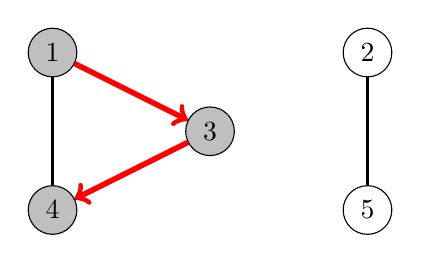
\begin{tikzpicture}
\node[draw, circle] (2) at (7,5) {$2$};
\node[draw, circle,fill=lightgray] (1) at (3,5) {$1$};
\node[draw, circle,fill=lightgray] (3) at (5,4) {$3$};
\node[draw, circle] (5) at (7,3) {$5$};
\node[draw, circle,fill=lightgray] (4) at (3,3) {$4$};

\path[draw,thick,-] (1) -- (3);
\path[draw,thick,-] (1) -- (4);
\path[draw,thick,-] (3) -- (4);
\path[draw,thick,-] (2) -- (5);

\path[draw=red,thick,->,line width=2pt] (1) -- (3);
\path[draw=red,thick,->,line width=2pt] (3) -- (4);

\end{tikzpicture}
\end{center}

由于搜索没有访问所有节点，
我们可以得出结论：该图不是连通的。
类似地，我们还可以找出图的所有连通分量，
方法是遍历所有节点，如果当前节点
还不属于任何分量，就启动一次新的深度优先搜索。

\subsubsection{寻找环}

\index{环}

如果在图的遍历过程中，我们发现某个节点的邻居（除了当前路径上的前一个节点之外）已经被访问过，则该图包含一个环。
例如，图
\begin{center}
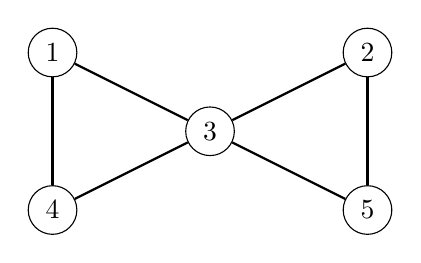
\begin{tikzpicture}
\node[draw, circle] (2) at (7,5) {$2$};
\node[draw, circle] (1) at (3,5) {$1$};
\node[draw, circle] (3) at (5,4) {$3$};
\node[draw, circle] (5) at (7,3) {$5$};
\node[draw, circle] (4) at (3,3) {$4$};

\path[draw,thick,-] (1) -- (3);
\path[draw,thick,-] (1) -- (4);
\path[draw,thick,-] (3) -- (4);
\path[draw,thick,-] (2) -- (5);
\path[draw,thick,-] (2) -- (3);
\path[draw,thick,-] (3) -- (5);
\end{tikzpicture}
\end{center}
包含两个环，我们可以按如下方式找到
其中一个：
\begin{center}
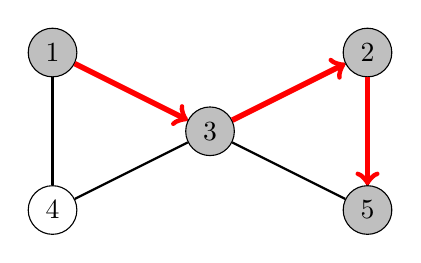
\begin{tikzpicture}
\node[draw, circle,fill=lightgray] (2) at (7,5) {$2$};
\node[draw, circle,fill=lightgray] (1) at (3,5) {$1$};
\node[draw, circle,fill=lightgray] (3) at (5,4) {$3$};
\node[draw, circle,fill=lightgray] (5) at (7,3) {$5$};
\node[draw, circle] (4) at (3,3) {$4$};

\path[draw,thick,-] (1) -- (3);
\path[draw,thick,-] (1) -- (4);
\path[draw,thick,-] (3) -- (4);
\path[draw,thick,-] (2) -- (5);
\path[draw,thick,-] (2) -- (3);
\path[draw,thick,-] (3) -- (5);

\path[draw=red,thick,->,line width=2pt] (1) -- (3);
\path[draw=red,thick,->,line width=2pt] (3) -- (2);
\path[draw=red,thick,->,line width=2pt] (2) -- (5);

\end{tikzpicture}
\end{center}
从节点 2 移动到节点 5 后，我们注意到
节点 5 的邻居 3 已经被访问过了。
因此，该图包含一个经过节点 3 的环，
例如，$3 \rightarrow 2 \rightarrow 5 \rightarrow 3$。

判断一个图是否包含环的另一种方法是
简单地计算每个连通分量中的节点数和边数。
如果一个连通分量包含 $c$ 个节点且没有环，
则它必须恰好包含 $c-1$ 条边
（即它必须是一棵树）。
如果有 $c$ 条或更多的边，则该连通分量
一定包含一个环。

\subsubsection{二分图检查}

\index{二分图}

如果一个图的节点可以用两种颜色着色，
使得没有相邻的节点具有相同的颜色，
则该图是二分图。
使用图的遍历算法可以非常容易地
检查一个图是否是二分图。

基本思路是将起始节点着为蓝色，
其所有邻居着为红色，邻居的邻居着为蓝色，依此类推。
如果在搜索过程中的某个时刻，我们发现
两个相邻的节点具有相同的颜色，
这意味着该图不是二分图。
否则，该图是二分图，并且已经找到了一种着色方案。

例如，图
\begin{center}
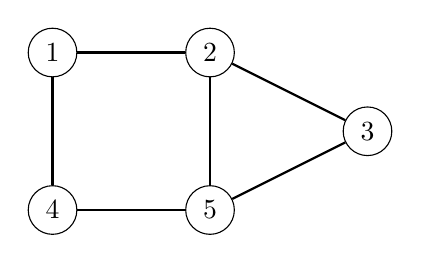
\begin{tikzpicture}
\node[draw, circle] (2) at (5,5) {$2$};
\node[draw, circle] (1) at (3,5) {$1$};
\node[draw, circle] (3) at (7,4) {$3$};
\node[draw, circle] (5) at (5,3) {$5$};
\node[draw, circle] (4) at (3,3) {$4$};

\path[draw,thick,-] (1) -- (2);
\path[draw,thick,-] (2) -- (5);
\path[draw,thick,-] (5) -- (4);
\path[draw,thick,-] (4) -- (1);
\path[draw,thick,-] (2) -- (3);
\path[draw,thick,-] (5) -- (3);
\end{tikzpicture}
\end{center}
不是二分图，因为从节点 1 开始的搜索
进行如下：
\begin{center}
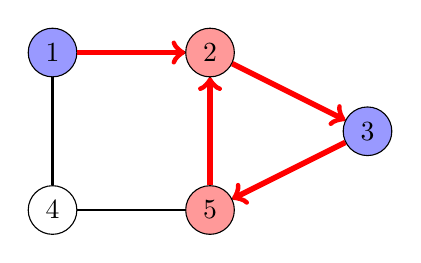
\begin{tikzpicture}
\node[draw, circle,fill=red!40] (2) at (5,5) {$2$};
\node[draw, circle,fill=blue!40] (1) at (3,5) {$1$};
\node[draw, circle,fill=blue!40] (3) at (7,4) {$3$};
\node[draw, circle,fill=red!40] (5) at (5,3) {$5$};
\node[draw, circle] (4) at (3,3) {$4$};

\path[draw,thick,-] (1) -- (2);
\path[draw,thick,-] (2) -- (5);
\path[draw,thick,-] (5) -- (4);
\path[draw,thick,-] (4) -- (1);
\path[draw,thick,-] (2) -- (3);
\path[draw,thick,-] (5) -- (3);

\path[draw=red,thick,->,line width=2pt] (1) -- (2);
\path[draw=red,thick,->,line width=2pt] (2) -- (3);
\path[draw=red,thick,->,line width=2pt] (3) -- (5);
\path[draw=red,thick,->,line width=2pt] (5) -- (2);
\end{tikzpicture}
\end{center}
我们注意到节点 2 和 5 的颜色
都是红色，而它们在图中是相邻的节点。
因此，该图不是二分图。

这个算法总是有效的，因为当只有
两种颜色可用时，一个连通分量中起始节点的颜色
决定了该分量中所有其他节点的颜色。
起始节点是红色还是蓝色
并没有任何区别。

注意，在一般情况下，
要判断一个图中的节点是否能用 $k$ 种颜色着色
使得没有相邻的节点具有相同的颜色
是很困难的。
即使当 $k=3$ 时，也没有已知的高效算法，
该问题是 NP 困难的。
